% author Truong Nhan Nguyen
% created in 4/1/2022

\documentclass[tikz, border=10pt]{standalone}

\usepackage{tikz}
\usetikzlibrary{mindmap, shadows}
\usepackage{xcolor}

\tikzset{
    every node/.style = {font=\footnotesize\sffamily\bfseries, circular drop shadow},
    level 1 concept/.append style = {level distance=20em, sibling angle=90},
    level 2 concept/.append style = {level distance=15em, sibling angle=60},
    level 3 concept/.append style = {level distance=8em, sibling angle=30}
}

\begin{document}
    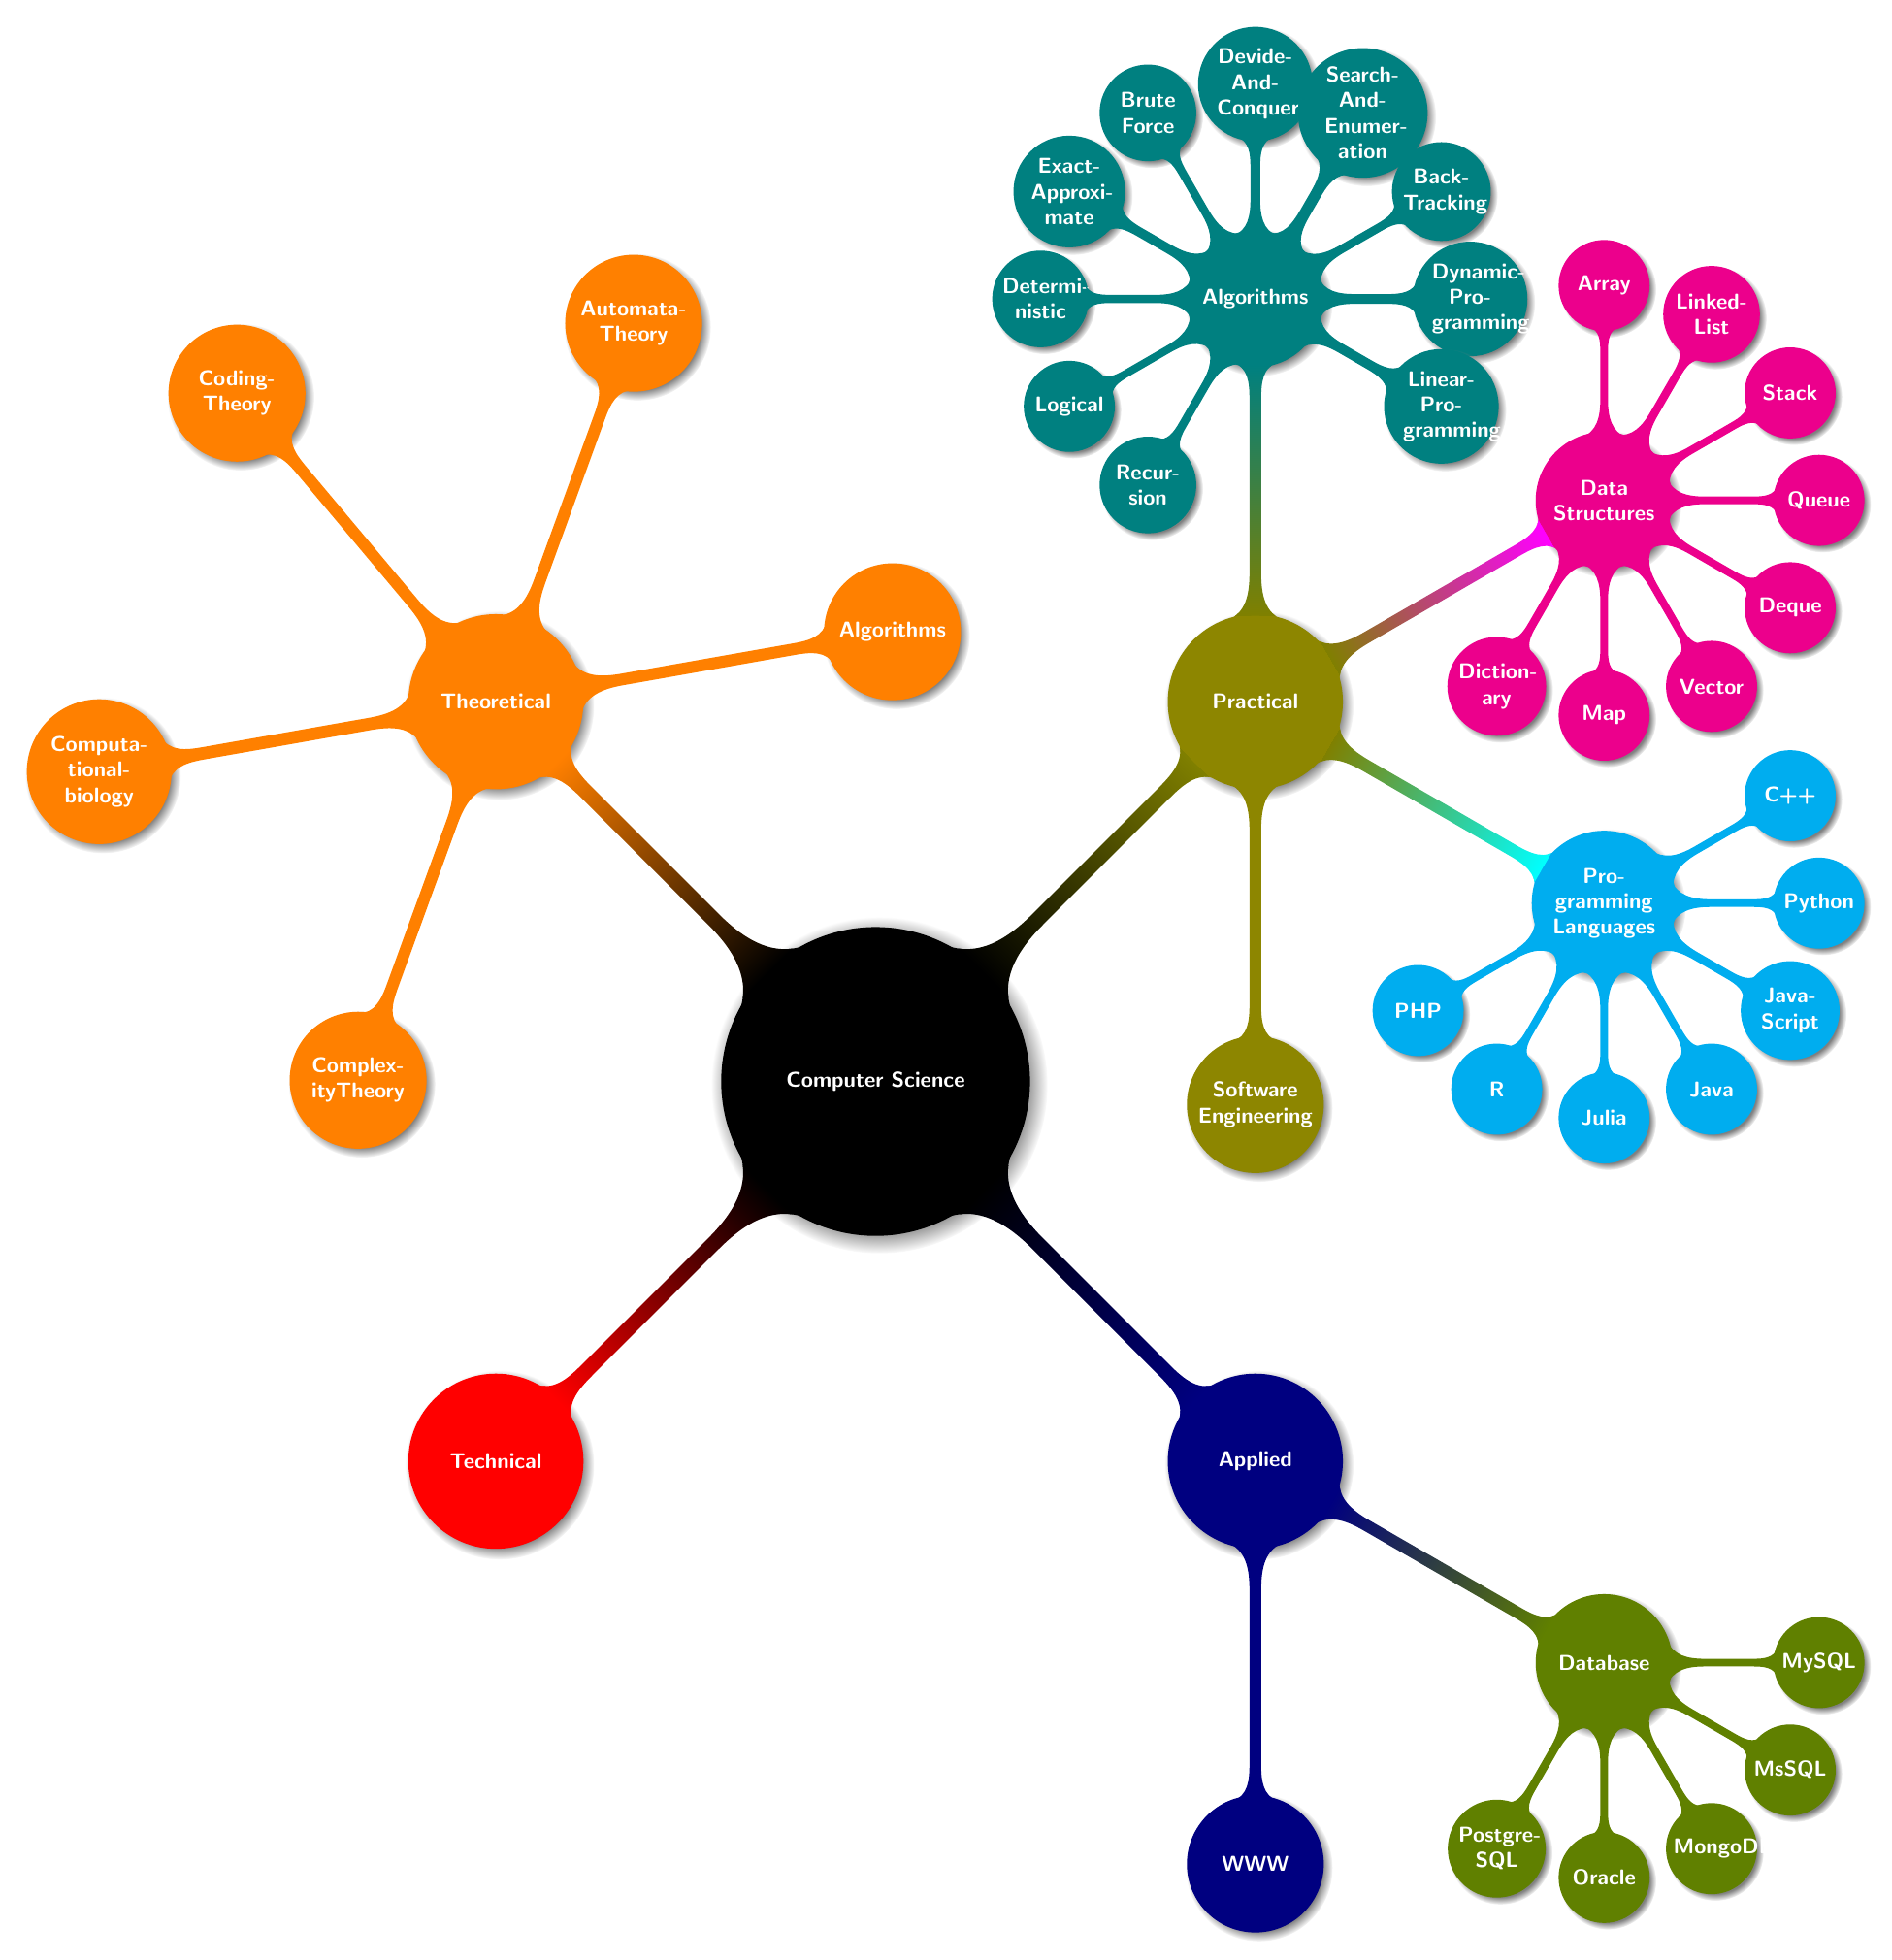
\begin{tikzpicture}
        \path[mindmap, concept color=black, text=white]
            node[concept]{Computer Science}
            [clockwise from=45]
                child[concept color=olive] {
                    node[concept] {Practical}
                    [clockwise from=90]
                    child[concept color=teal] {
                        node[concept] {Algorithms}
                        [clockwise from=240] 
                            child {node[concept] {Recur\-sion}}
                            child {node[concept] {Logical}}
                            child {node[concept] {Determi\-nistic}}
                            child {node[concept] {Exact\-Approxi\-mate}}
                            child {node[concept] {Brute Force}}
                            child {node[concept] {Devide\-And\-Conquer}}
                            child {node[concept] {Search\-And\-Enumer\-ation}}
                            child {node[concept] {Back\-Tracking}}
                            child {node[concept] {Dynamic\-Pro\-gramming}}
                            child {node[concept] {Linear\-Pro\-gramming}}
                    }
                    child[concept color=magenta] {
                        node[concept] {Data Structures}
                        [clockwise from=90]
                            child {node[concept] {Array}}
                            child {node[concept] {Linked\-List}}
                            child {node[concept] {Stack}}
                            child {node[concept] {Queue}}
                            child {node[concept] {Deque}}
                            child {node[concept] {Vector}}
                            child {node[concept] {Map}}
                            child {node[concept] {Diction\-ary}}
                    }
                    child[concept color=cyan] {
                        node[concept] {Pro\-gramming Languages}
                        [clockwise from=30]
                            child {node[concept] {C++}}
                            child {node[concept] {Python}}
                            child {node[concept] {Java\-Script}}
                            child {node[concept] {Java}}
                            child {node[concept] {Julia}}
                            child {node[concept] {R}}
                            child {node[concept] {PHP}}
                    }
                    child {node[concept] {Software Engineer\-ing}}
                }
                child[concept color=blue!50!black] {
                    node[concept] {Applied}
                    [clockwise from=-30]
                    child[concept color=lime!50!black] {
                        node[concept] {Database}
                        [clockwise from=0]
                            child {node[concept] {MySQL}}
                            child {node[concept] {MsSQL}}
                            child {node[concept] {MongoDB}}
                            child {node[concept] {Oracle}}
                            child {node[concept] {Postgre\-SQL}}
                    }
                    child {node[concept] {WWW}}
                }
                child[concept color=red] {
                    node[concept] {Technical}
                }
                child[concept color=orange] {
                    node[concept] {Theoretical}
                    [counterclockwise from=10]
                        child {node[concept] {Algo\-rithms}}
                        child {node[concept] {Automata\-Theory}}
                        child {node[concept] {Coding\-Theory}}
                        child {node[concept] {Computa\-tional\-biology}}
                        child {node[concept] {Complex\-ity\-Theory}}
                };
    \end{tikzpicture}
\end{document}